\section{Methods}
\subsection{Data Description}
We used the Yelp Open Dataset, which contains more than 8.6 million reviews for approximately 160,000 businesses\cite{b4} and is publicly available on the web\cite{b5}. The dataset includes posts from October 2004 to January 2021, but we analyzed approximately 2.5 million reviews. For this project, we limited our scope to the top 5 cities with the most POIs count (Table 1). We also reviewed around 5 million checkins and used it to get activity in the city (Section B.)
We found that the median number of reviews per business is 15, and the mean is 42.5. Although 31\% of points of interest (POIs) have fewer than 10 reviews, a few outliers have many reviews. We also observed that around 20\% of businesses had no relationship words in their reviews, and over two-thirds of businesses had fewer than five relationship word occurrences total, which could be due to few total reviews. In later sections, we normalized the relationship word count for each business to get the expected word count per 1,000 reviews, which we called the relationship word rate. To avoid spurious or insignificant results, we only considered POIs with at least 30 reviews and at least 30 relationship-word occurrences.

\begin{table}[htbp]
  \renewcommand{\arraystretch}{1.2}
  \caption{Summary of POI and check-in statistics by city}
  \label{table:poi_stats}
  \centering
  \begin{tabular}{|p{1.3cm}|p{1cm}|p{1cm}|p{1cm}|p{1cm}|p{1cm}|}
    \hline
    \textbf{City} & \textbf{\# POIs} & \textbf{Total Reviews} & \textbf{Median Reviews per POI} & \textbf{Total Check-ins} & \textbf{Median Check-ins per POI} \\
    \hline
    Philadelphia & 14,569 & 813,634 & 17 & 1,838,206 & 17 \\
    \hline
    Tucson & 9,250 & 321,269 & 12 & 772,140 & 13 \\
    \hline
    Tampa & 9,050 & 359,167 & 13 & 918,203 & 16 \\
    \hline
    Indianapolis & 7,540 & 289,986 & 13 & 886,001 & 22 \\
    \hline
    Nashville & 6,971 & 361,162 & 15 & 817,283 & 18 \\
    \hline
  \end{tabular}
\end{table}

We used the Yelp Fusion API Category List\cite{b9} to assign each Point of Interest (POI) to one or more of the 22 top-level categories. However, we considered only businesses within eight categories that were likely to provide a place for social activity, as listed in Table 2. Table 2 is a break down of POIs in top 5 cities mentioned in Table 1. We excluded categories such as "Home Services" (e.g., plumbing, pool cleaners, etc.) that were unlikely to offer social spaces. We note that there is a distinction between "Restaurants" and "Food". "Restaurants" refers to sit-down establishments, while "Food" includes other places where food and drinks are sold, such as coffee shops and food trucks.

\begin{table}[h]
    \centering
    \caption{Number of POIs in each category}
    \small
    \begin{tabular}{|l|r|}
        \hline
        Category & Number of POIs \\
        \hline
        Restaurants & 19133 \\
        Shopping & 9639 \\
        Beauty \& Spas & 6210 \\
        Food & 4942 \\
        Active Life & 3350 \\
        Hotels \& Travel & 2009 \\
        Arts \& Entertainment & 1630 \\
        Nightlife & 1298 \\
        \hline
    \end{tabular}
    \label{tab:businesses}
\end{table}

Relationship keywords were sourced from the American Time Use Survey\cite{b7}, we also used colloquial keywords such as "bae", "boo", and "roommate". Following the methodology of prior work\cite{b2}, the resulting words were grouped into four categories: family, romantic, friendship, and professional (Table 3), according to interpersonal relationship types from sociology and business management sectors. To avoid the need for word stemming during text mining, multiple forms of each relationship word were added to the list (e.g., "friend" and "friends"). The final list of relationship keywords is shown in Table 3, which includes words such as "bff", "partner", "coworker", and "spouse".

\begin{table}[htbp]
    \centering
    \caption{Relationship Keywords}
    \begin{tabular}{|p{1.5cm}|p{6.5cm}|}
    \hline
    \textbf{Type} & \textbf{Words} \\
    \hline
    Family & child(ren), kid(s), daughter(s), son(s), parent(s), mother, mom, father, dad, brother(s), sister(s), siblings, aunt(s), uncle(s), niece(s), nephew(s), cousin(s), grandchild(ren), grandmother, grandma, grandfather, grandpa, grandparents \\
    \hline
    Romantic & partner, relationship, date, boo, bae, sweetheart, fiance, fiancee, girlfriend, gf, boyfriend, bf, spouse, husband, wife \\
    \hline
    Friendship & bff, friend(s), buddy, buddies, pal(s), housemate(s), roommate(s), flatmate(s) \\
    \hline
    Professional & neighbor(s), classmate(s), teacher(s), coworker(s), colleague(s), client(s), boss \\
    \hline
    \end{tabular}
\end{table}

\subsection{Analytical Methods}

\textbf{Scalar function}, that is used in this work, is the
density function. The input data Yelp is provided as a set of
points (data points) having location and time. The density function at
a given location p is defined as the Gaussian weighted sum of data points xi
that are in its neighborhood N(p). Here d() is the Euclidean distance between two points, and $\epsilon$ is the extent of the influence region for a given data point. The neighborhood N(p) is defined
as a circular region centered at p. 

\begin{equation}
f(p) = \sum\limits_{x_i\in N(p)} e^{-\frac{d(p,x_i)^2}{\epsilon^2}}
\end{equation}

In order to efficiently compute the topological features of the scalar function f , it is represented as piecewise linear (PL) function f : K →
R. The planar domain D of the function is represented by a triangular mesh K. The function is defined on the vertices of the mesh and linearly interpolated within each triangle.
To take into account the variation with time, the set of data points
are first grouped together into a discrete set of time steps corresponding to the temporal resolution, and the scalar function is computed for each of these time steps.

\textbf{POI Categorization}: To identify the prevalence of relationship words in Yelp reviews, we employed several preprocessing steps. First, we converted all words to lowercase and replaced punctuation marks with spaces, as reviews often contain possessive forms of words. We then utilized a two-word tokenization approach to identify relationship words preceded by the words "my" or "our" (in cases related to children), as this helped to avoid instances where authors were not referring to their own relationships. Additionally, this approach helped to address the edge cases of POIs with relationship words in their names. We removed any duplicate tokens within individual reviews to capture the overall prevalence of relationship words across reviews, rather than within them. After counting the occurrences of relationship keywords per POI, we calculated the z-scores and p-values to determine the confidence values for each POI. Cdf is cumulative distribution function of the standard normal distribution.

\begin{equation}
\begin{aligned}
\quad z &= \frac{x-\mu}{\sigma}\
\quad p &= 2 * (1 - cdf(z))\
\quad conf &= (1 - p) * 100
\end{aligned}
\end{equation}

This enabled us to more accurately identify businesses with higher or lower-than-expected use of relationship words in their reviews, and gain insights into how people talk about different types of businesses.

\textbf{POI to Pulse Mapping}: In order to map the existing Yelp points of interest (POIs) to urban pulses, it is essential to first determine the critical points using check-in data from the Yelp dataset. Once the critical points (section 2.4) are identified, we proceed to map the POIs using a clustering approach. We map the POIs to the critical point if they are within a user-specified influence region, known as an $\epsilon$-distance, of each other. (Fig 2.) The same $\epsilon$-distance is used for computing the density function in the previous section. After the locations are identified and clustered, they are categorized into three types of beats that capture variations over time\cite{b1}. These beats represent scalar functions that aggregate the data and not the raw data itself. The beats are defined for each possible temporal resolution, thereby enabling a better understanding of how the prominent POIs behave at different times and resolutions.

\begin{figure}
    \centering
    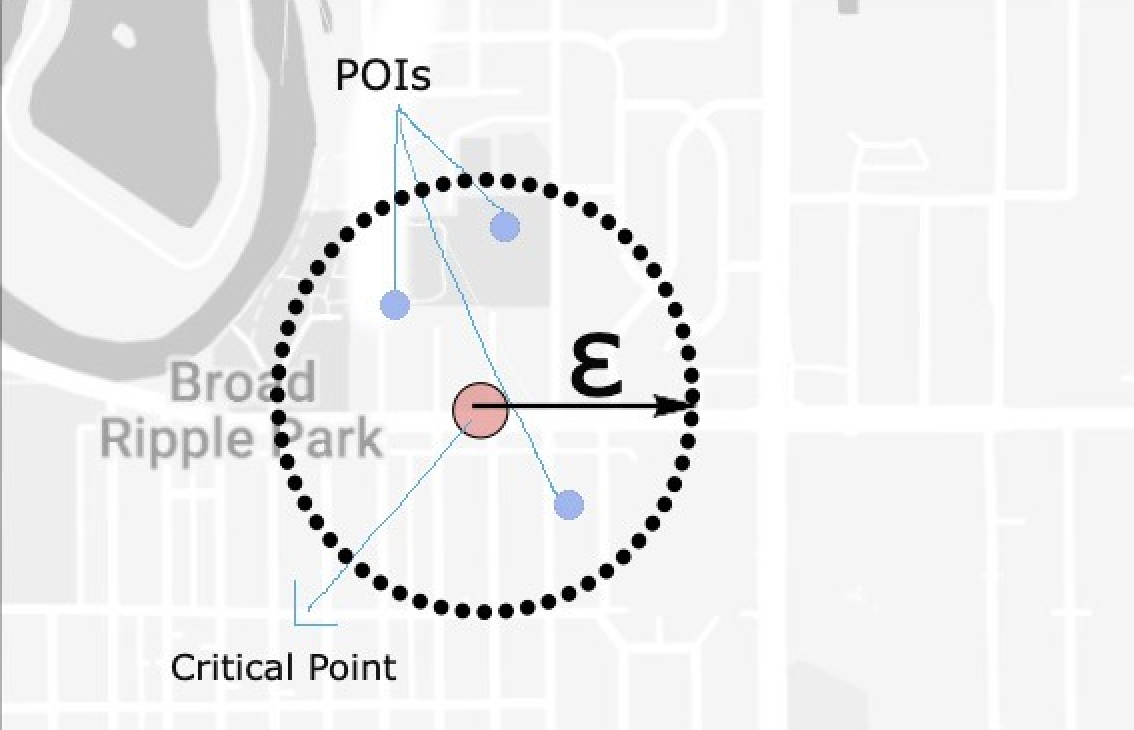
\includegraphics[width=8cm, height=5cm]{Image1.png}
    \caption{Critical Point and POIs within $\epsilon$-distance}
    \label{fig:my_label}
\end{figure}
